\section{Proposed model} \label{proposed_model}

	\subsection{Experimental enviroment}
	
	Training a deep learning model that involves intensive compute tasks on large dataset can take days to run on a single CPU or a slow GPU. In our case, since HAM10000 dataset has 10015 images, it was unthinkable to perform the training of a convolutional neural network with a standard laptop. The solution turned to cloud computing. The choice has fallen on Google Cloud Platform for the availability of a free tier that consists in 300\$ free credits that can be used in any GCP product. 
	
	\smallskip
	
	We have tested our CNN models on a custom instance of Compute Engine. Our VM's configuration is presented in Table \ref{tab:hw-config}.
	
	\begin{table}[H]
		\centering
		\begin{tabular}{ |c|c|c|c|c|c| }
			\hline
			\textbf{Operating System} & \textbf{CPU} & \textbf{Memory} & \textbf{Disk} & \textbf{GPU} \\ \hline
			
			Ubuntu 18.04 LTS & 8 core & 52 GB & SSD / 100 GB & 1x NVIDIA Tesla K80 \\ \hline
			
		\end{tabular}
		\caption{Virtual machine configuration}
		\label{tab:hw-config}
	\end{table}
	
	Our models have been implemented in Keras using tensorflow as a backend. The code is available on our GitHub repository: \url{https://github.com/albertobezzon/cognitiveservices}.

	\subsection{Performance measures choice}
		
		As mentioned in Section \ref{dataset}, HAM10000 is a highly imbalanced dataset and it has been a challenge to deal with it. The first problem we faced was on the choice of the right performance measures for our experiments. Accuracy is usually referred as the best performance measure for image classification tasks but in case of imbalanced data is definitely not the right choice. In fact, if the accuracy is high it does not mean that we have found a good model, because it can be possible that it is high only because our model is very good in predicting majority classes, but we want our model to be accurate on all the classes, even the most challenging minority classes.
		
		\smallskip
		
		Our goal is to obtain a model that maximize both precision and recall on all the classes.
		To achieve this goal, we have decided to use F1-measure and macro average performance measures. F1-measure allows to understand in which classes our model performs well: a high F1 score for one class means that our model returns a high precision but also a high recall on that specific class. 
		
		\smallskip
		
		We have then selected the macro average F1 because we are interested in knowing if our model performs well in minority classes, which include malign skin cancers, such as Melanoma class, that is the most important one in the dataset. 
		Moreover, if the model performs well in minority classes, even if the number of examples is limited, means that it is able to learn the correct features to discriminate between these classes. 
		
		\smallskip
		
		Finally, since we are interested in predicting well malign skin cancers, we did not use micro average because it returns high scores when the model performs well in majority classes, which include benign tumors.
		
	\subsection{Transfer learning attempt}
		
		As mentioned in Section \ref{related_works}, we firstly tried to apply transfer learning on our task. We took Inception v3 model, pre-trained on ImageNet Challenge, and we then changed the classification part on top of it with a custom classifier. This classifier was composed of one global average pooling layer, two fully connected layers and finally a softmax layer. We took this architecture from \cite{article2} because they had obtained the best results we have found on HAM10000. We froze all the layers except of the custom classification part and we trained our model with the settings reported in \cite{article2}. We obtained bad performances with this model compared to the performances reported in the paper. The accuracy was relatively high (67\%) but when we moved to the confusion matrix we discovered that the model was predicting everything like a Melanocytic nevi to maximize the overall accuracy. So, the model was not able to learn anything. After this test we decided to move to the classic CNN architecture, in fact transfer learning performs well when the dataset is similar to the ImageNet dataset and it was not the case.
		
	\subsection{Proposed model architecture}
	
		For the design of our CNN model architecture we have followed a common design pattern in CNNs. This pattern consists in building a simple model architecture with only one convolutional block and to increase its depth until the adding of a new convolutional block does not give better performances compared to the last model built. We proceeded this way because we found that this pattern performs well in general image classification tasks and the experiments in \cite{article3} showed that it performs well even in skin cancer classification task. So, we began our project with the construction of a base model that we have then tried to improve. In Figure \ref{fig:base_model} we present our base model. Its architecture is composed of a convolutional block and a simple classification block, which are the building blocks of modern CNN architectures. The convolutional block is composed of two convolutional layers with 32 activation maps followed by a max pooling layer. We have decided to set a 3x3 filter size for the convolutional layers because local features in skin lesions are relatively small. The classification block is composed of a flatten layer used to flat the output of the convolutional block, a fully connected layer with 64 units and finally a softmax layer. We have then added a dropout layer after the fully connected layer. We will explain our regularizations techniques in Section \ref{regularization_techniques}. 
		
		\begin{figure}[H]
			\centering
			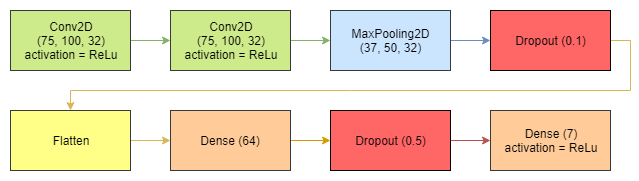
\includegraphics[width=15cm]{images/base_model.png}
			\caption{Base model architecture}
			\label{fig:base_model}
		\end{figure}
	
		Given the base model we began to add convolutional blocks to it to see if model performances increased. The adding of a convolutional block consists in add two convolutional layers with doubled activation maps followed by a max pooling layer after the previous convolutional block of the network. With this technique we have changed the architecture of our base model five times until we obtained our best and proposed model. In Table \ref{tab:models_performances} is possible to compare the performances of the models we have tried. The table presents the F1 scores for all the classes, the macro average of the F1 score and the test accuracy for each model. We trained these models with the settings reported in Section \ref{training_settings}.
		
		\begin{table}[H]
			\small
			\begin{threeparttable}
				\begin{tabular}{ |>{\centering\arraybackslash}p{2cm}|c|c|c|c|c|c|c|>{\centering\arraybackslash}p{2cm}|>{\centering\arraybackslash}p{2cm}| }
					\hline
					\textbf{Model} & \textbf{akiec} & \textbf{bcc} & \textbf{bkl} & \textbf{df} & \textbf{mel} & \textbf{nv} & \textbf{vasc} & \textbf{Macro average} & \textbf{Test accuracy} \\ \hline
					
					Base model\tnotex{tnote:model1} & 0.32 & 0.45 & 0.47 & 0.13 & 0.34 & 0.87 & 0.49 & 0.44 & 0.74 \\ \hline
					Model 2\tnotex{tnote:model2} & 0.40 & 0.53 & 0.50 & 0.00 & 0.36 & 0.88 & 0.72 & 0.48 & 0.76 \\ \hline
					Model 3\tnotex{tnote:model3} & 0.38 & 0.52 & 0.52 & 0.07 & 0.47 & 0.89 & 0.58 & 0.49 & 0.77 \\ \hline
					Proposed model\tnotex{tnote:model4} & 0.41 & 0.52 & 0.53 & 0.16 & 0.38 & 0.90 & 0.65 & 0.51 & 0.76 \\ \hline
					Model 5\tnotex{tnote:model5} & 0.34 & 0.46 & 0.53 & 0.07 & 0.39 & 0.90 & 0.62 & 0.47 & 0.75 \\ \hline
					
				\end{tabular}		
				\begin{tablenotes}
					\item\label{tnote:model1} $2 x Conv2D(32) \rightarrow MaxPool2D \rightarrow Dropout(0.1) \rightarrow Flatten \rightarrow FC(64) \rightarrow Dropout(0.5) \rightarrow Softmax(7)$
					\item\label{tnote:model2} $2 x Conv2D(32) \rightarrow MaxPool2D \rightarrow Dropout(0.1) \rightarrow 2 x Conv2D(64) \rightarrow MaxPool2D \rightarrow Dropout(0.2) \rightarrow Flatten \rightarrow FC(128) \rightarrow Dropout(0.5) \rightarrow Softmax(7)$
					\item\label{tnote:model3} $2 x Conv2D(32) \rightarrow MaxPool2D \rightarrow Dropout(0.1) \rightarrow 2 x Conv2D(64) \rightarrow MaxPool2D \rightarrow Dropout(0.2) \rightarrow 2 x Conv2D(128) \rightarrow MaxPool2D \rightarrow Dropout(0.3) \rightarrow Flatten \rightarrow FC(256) \rightarrow Dropout(0.5) \rightarrow Softmax(7)$
					\item\label{tnote:model4} $2 x Conv2D(32) \rightarrow MaxPool2D \rightarrow Dropout(0.1) \rightarrow 2 x Conv2D(64) \rightarrow MaxPool2D \rightarrow Dropout(0.2) \rightarrow 2 x Conv2D(128) \rightarrow MaxPool2D \rightarrow Dropout(0.3) \rightarrow 2 x Conv2D(256) \rightarrow MaxPool2D \rightarrow Dropout(0.4) \rightarrow Flatten \rightarrow FC(512) \rightarrow Dropout(0.5) \rightarrow Softmax(7)$
					\item\label{tnote:model5} $2 x Conv2D(32) \rightarrow MaxPool2D \rightarrow Dropout(0.1) \rightarrow 2 x Conv2D(64) \rightarrow MaxPool2D \rightarrow Dropout(0.2) \rightarrow 2 x Conv2D(128) \rightarrow MaxPool2D \rightarrow Dropout(0.3) \rightarrow 2 x Conv2D(256) \rightarrow MaxPool2D \rightarrow Dropout(0.4) \rightarrow 2 x Conv2D(512) \rightarrow MaxPool2D \rightarrow Dropout(0.5) \rightarrow Flatten \rightarrow FC(1024) \rightarrow Dropout(0.5) \rightarrow Softmax(7)$
				\end{tablenotes}
			\end{threeparttable}
			\caption{Models' performances}
			\label{tab:models_performances}
		\end{table}
	
		The base model has the worst performances compared to the other models. Model 2 increases the performances of the base model on all the classes, but it has the problem to be bad in classifying Dermatofibromas.
		Model 3 has the best accuracy on the test set but a macro average that is less than our proposed model and we prefer to balance the number of correct classifications over the classes instead of increasing the overall accuracy. 
		Even if model 3 has the best performances on melanoma detection we chose model 4 because we think it is able to capture more complex features on the images, in fact it has the highest F1 score in Dermatofibroma class, that seems to be the most difficult to classify for our models, and also it outperforms the other models on all the other classes. We think that our proposed model can reached these performances thanks to the number of convolutional blocks on it, in fact more convolutional blocks a network has and more complex features on the images will be able to detect. Moreover, we observed that model 4 has reached the maximum depth for our CNN in this specific task, in fact the adding of another convolutional block decreases most of the metrics scores.
		Finally, every time we added a new convolutional block we doubled also the number of units in the fully connected layer at the top of the network. We chose this strategy because more complex are the features that the convolution block is able to identify and more units in the fully connected layer will be required to capture these complex features.
		
		In Figure \ref{fig:proposed_model} we present the proposed model architecture. It performs well on HAM10000 compared to transfer learning and it has the advantage of the simplicity in the architecture. It is less depth and it takes faster training times thanks to the smaller number of parameters to be learnt. 
		After we have found the best architecture for this task we tried to do some experiments to increase its performances, such as class weighting and oversampling with data augmentation to deal with the problem of imbalanced data. In Section \ref{experiments} we present these experiments.
		
		\begin{figure}[H]
			\centering
			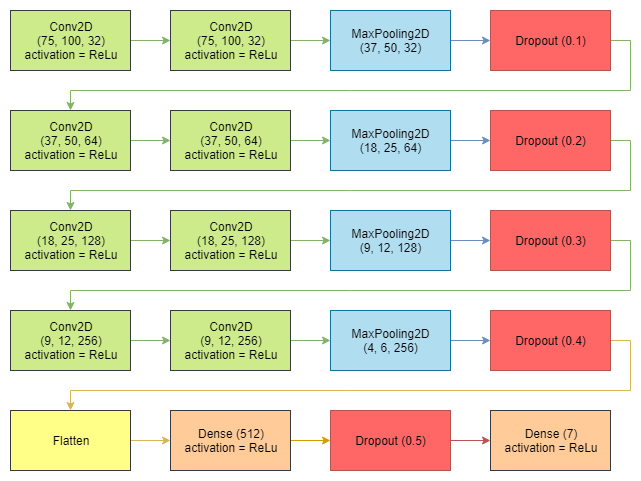
\includegraphics[width=15cm]{images/proposed_model.png}
			\caption{Proposed model architecture}
			\label{fig:proposed_model}
		\end{figure}
	
	\subsection{Regularization techniques and training settings}
	
		\subsubsection{Regularization techniques} \label{regularization_techniques}
		
			To prevent overfitting in our models we decided to use three common regularization techniques:
			
			\begin{itemize}
				\item \textbf{Dropout layers:} in previous section we presented our model architecture and it presents five dropout layers. The dropout layer after the fully connected layer freezes half of the units at each epoch. We set this high percentage because it is well known that fully connected layers are highly subject to overfitting. We then decided to add a dropout layer after each convolutional block, with an increasing percentage of frozen units. Since the number of parameters to be learnt increases with the increase of the depth of the network, this configuration helped our network to mitigate the overfitting issue;
				\item \textbf{Learning rate decay:} we set our model to decay the learning rate if no improvements on the validation accuracy are showed after 3 epochs of training. We tried many experiments and we discovered that this configuration helped the network avoids overfitting;
				\item \textbf{Early stopping:} since dropout and learning rate decay were not enough to avoid overfitting, early stopping was the next choice. Our models are configured to stop the learning in case of high overfitting. If the validation accuracy does not increase in 10 epochs, the training will be stopped and the weights corresponding to the best validation accuracy will be restored. We decided this configuration because we observed that in many cases the model needed many epochs to continue to learn.
			\end{itemize}
		
		\subsubsection{Optimizer and optimizer hyperparameters choice}
			
			We have tried three optimizers for the gradient descent: Stochastic Gradient Descent, RMSprop and Adam optimizers. We limited the test to these three optimizers because we found they are commonly used in skin cancer classification tasks. SGD and RMSprop did not perform well on our task. They did not allow the network to train, in fact the validation accuracy was stuck at 68\%. We had the same problem of transfer learning. We then tried Adam optimizer and the network began to learn.
			
			\smallskip
			
			We have selected only the learning rate of the Adam optimizer and we left all the other parameters at their default. We tried to train our models with a 0.001 learning rate. We have found that is the common choice in computer vision, but in our case the learning was too fast and the network began to overfit soon. We tried 0.00001 learning rate and we observed that the convergence was very stable, in fact the training accuracy and the validation accuracy followed the same behavior, but models took too much epochs to converge and very often the early stopping stopped the training even if there was not overfitting because 10 epochs were not enough to improve the training accuracy.
			
			\smallskip
			
			Finally, we have selected 0.0001 learning rate because we observed it was the best tradeoff between convergence speed and overfitting.
			In Figure \ref{fig:val_acc_lr} we show how training and validation accuracy behaviours change with the change of the learning rate.
			
			\begin{figure}[H] 
				\subfloat[Learning rate 0.001]{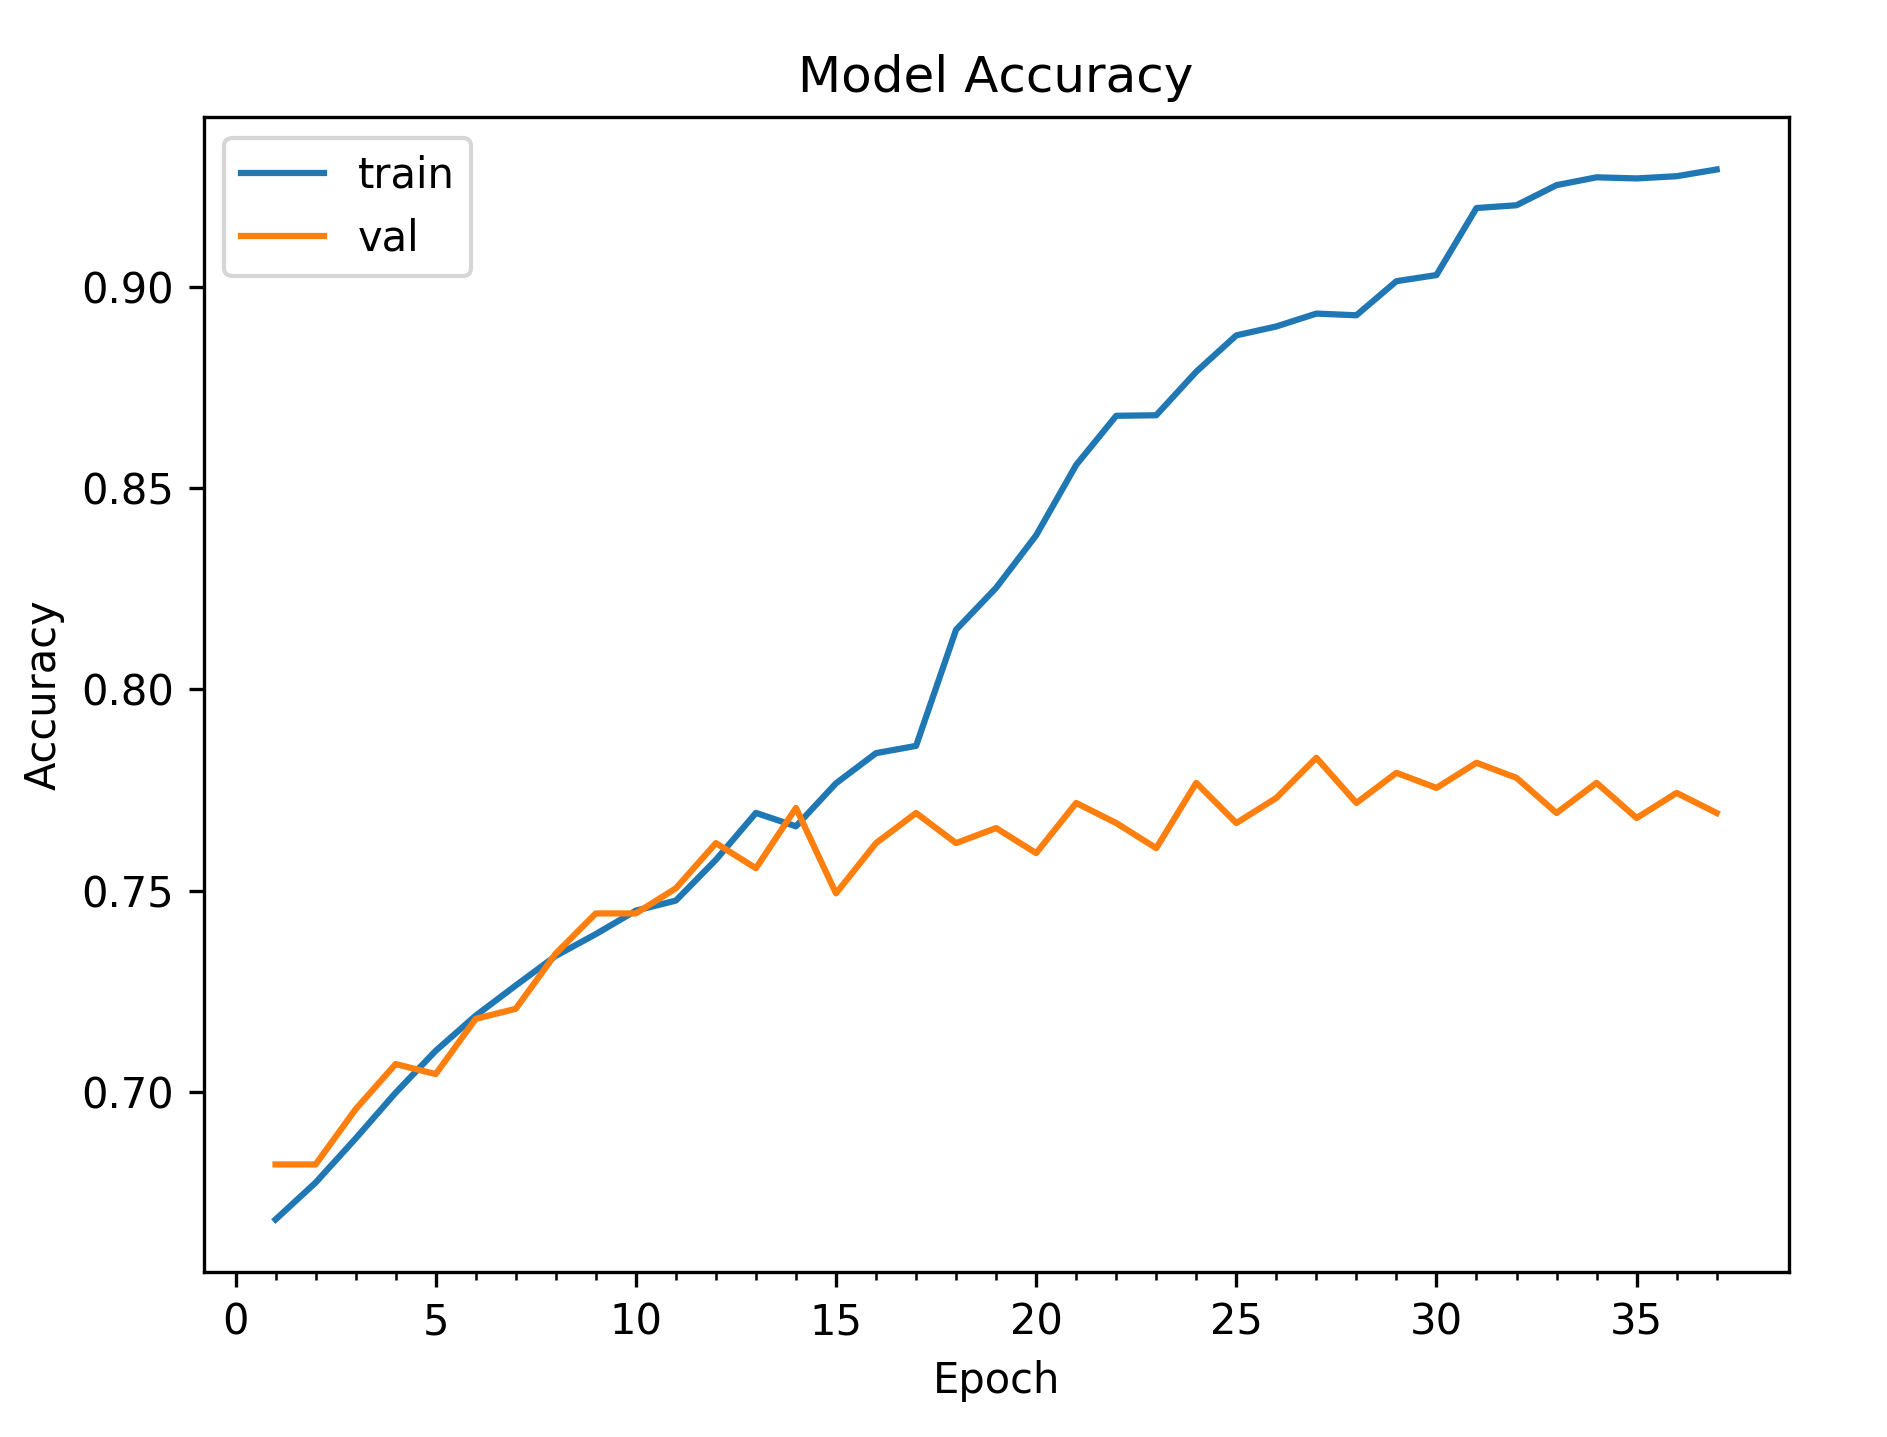
\includegraphics[width=0.33\columnwidth]{images/accuracy-loss-001.png}}
				\hspace*{\fill}
				\subfloat[Learning rate 0.00001]{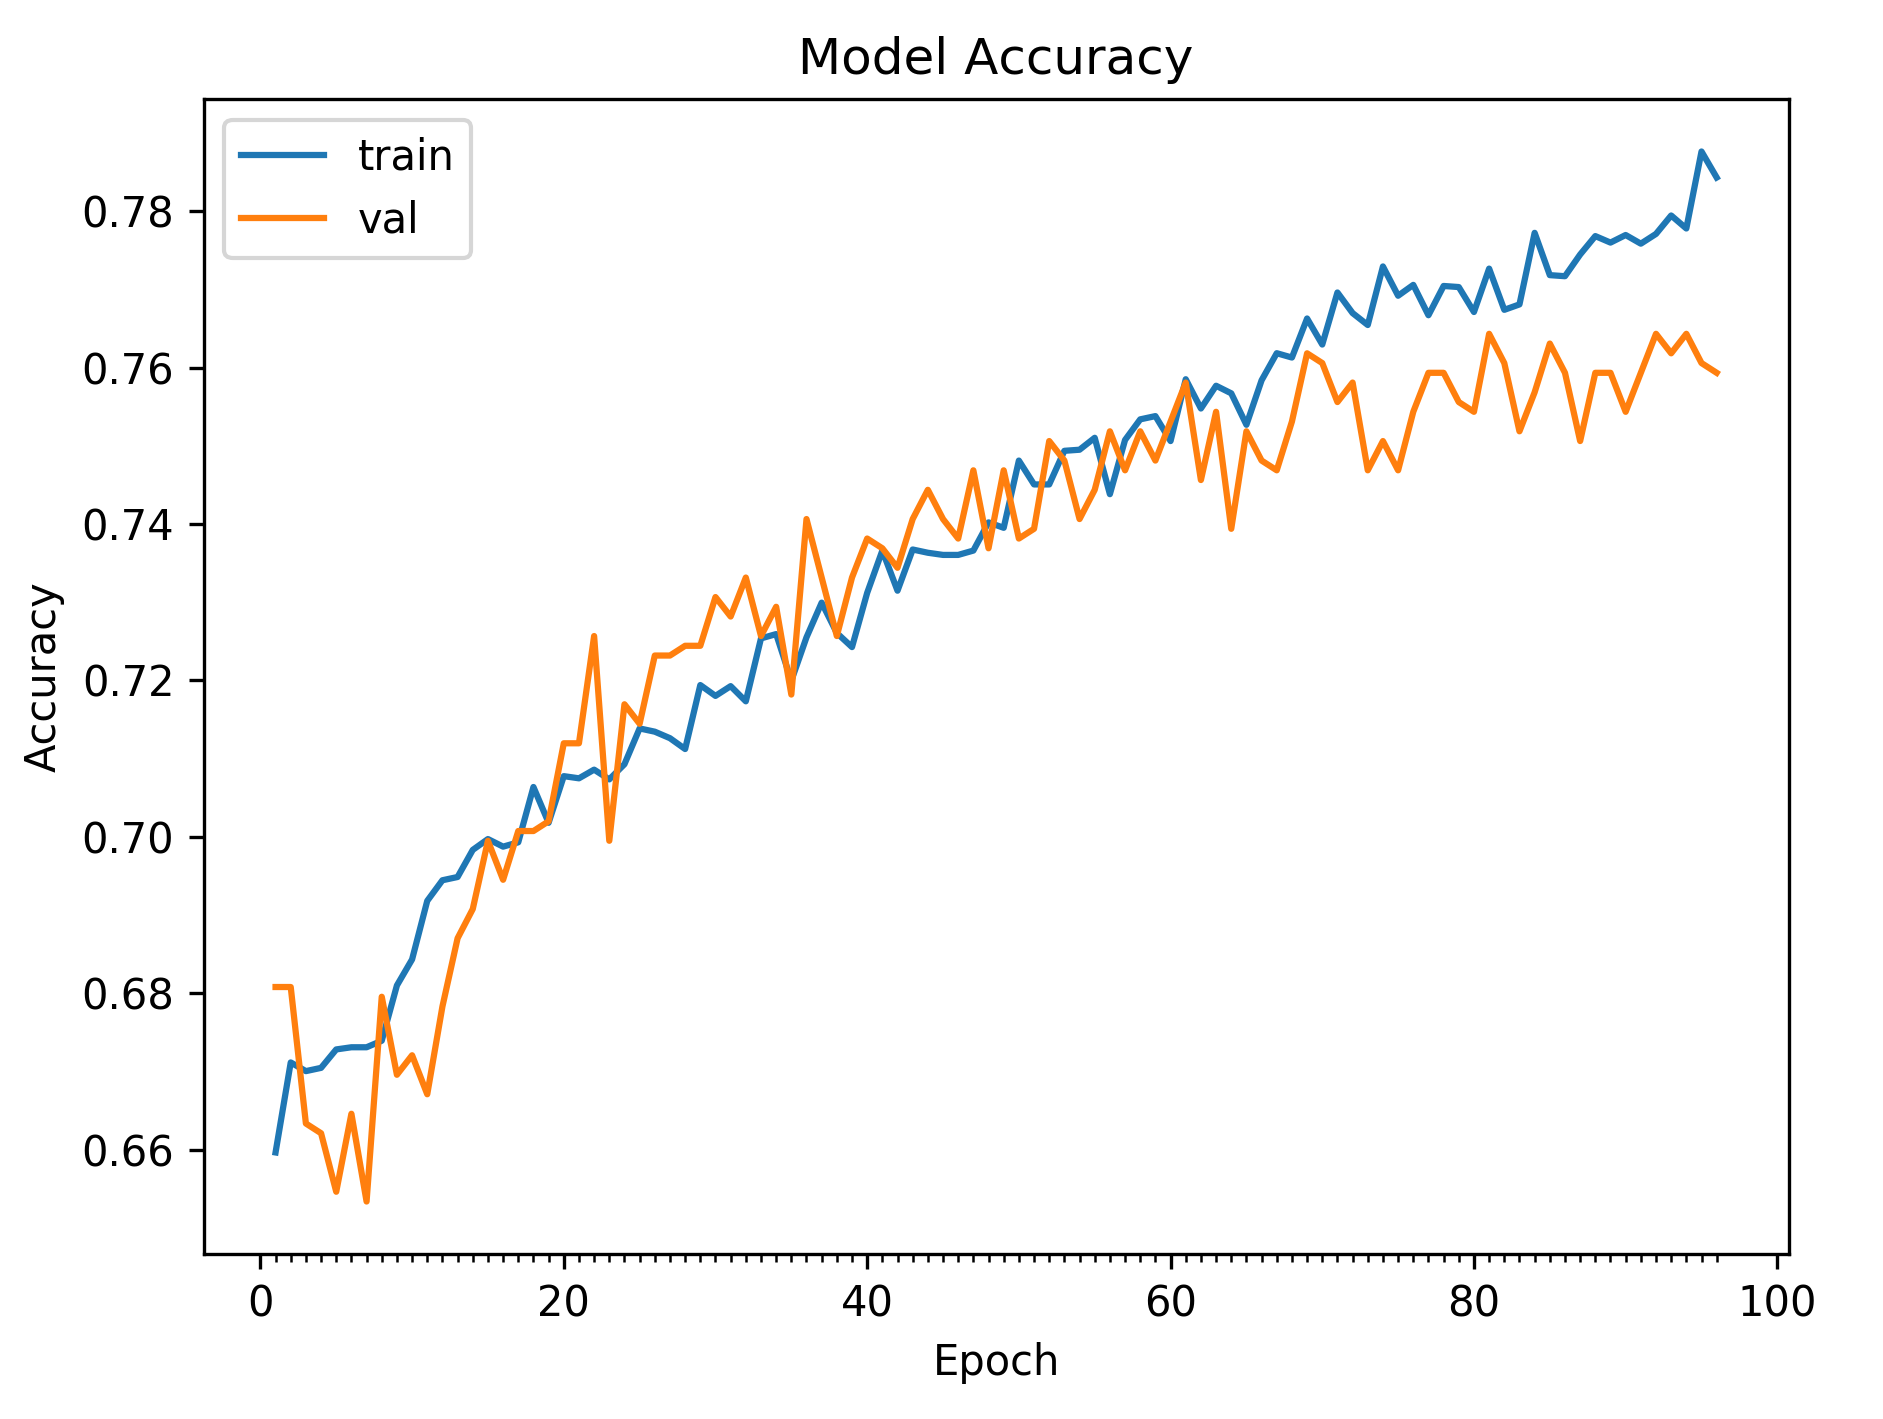
\includegraphics[width=0.33\columnwidth]{images/accuracy-loss-00001.png}}
				\hspace*{\fill}
				\subfloat[Learning rate 0.0001]{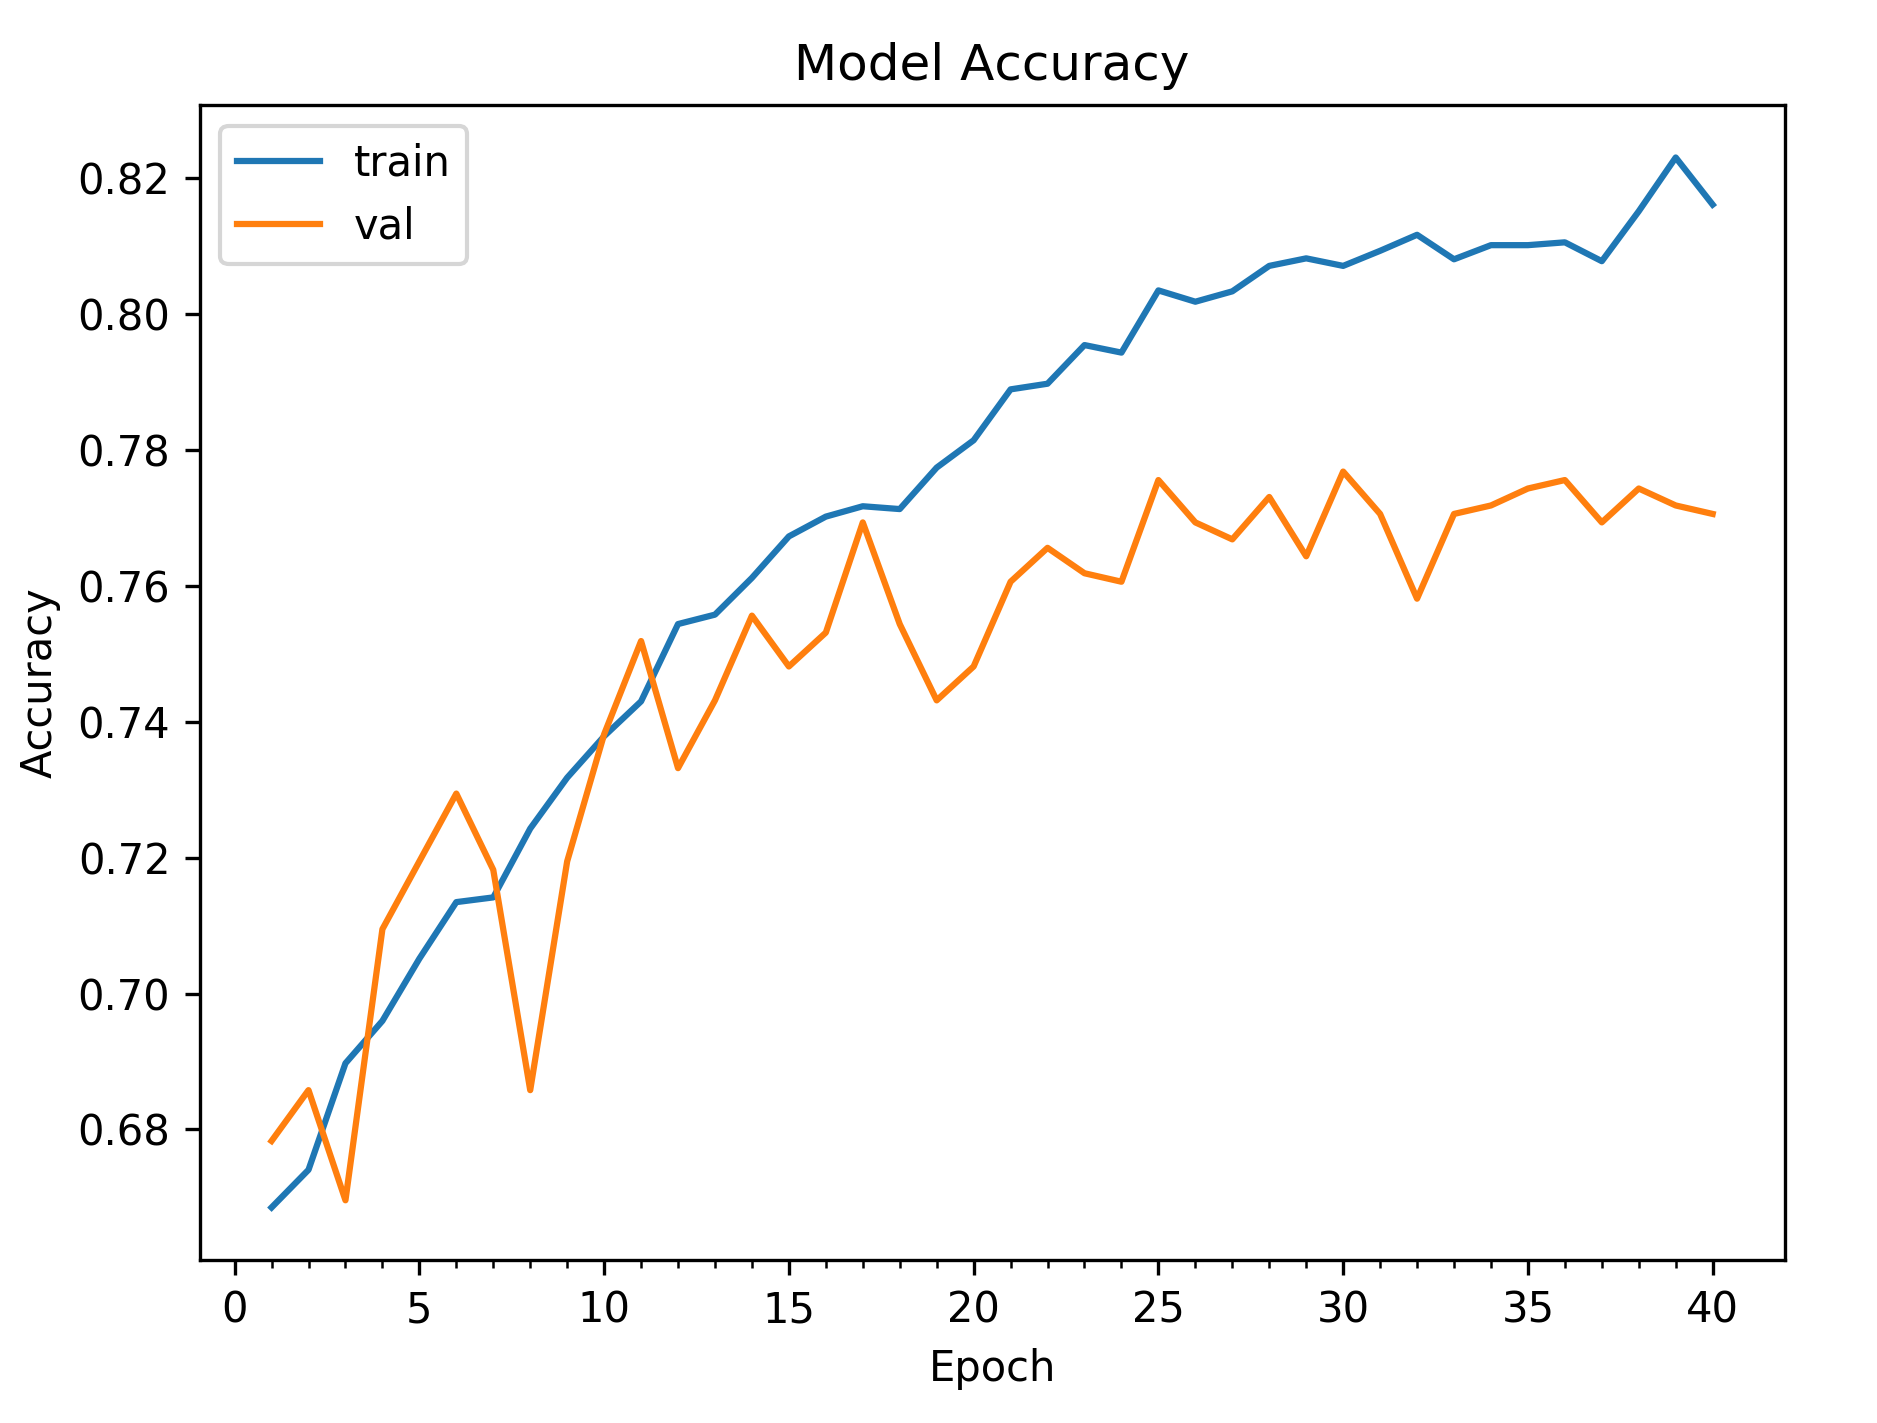
\includegraphics[width=0.33\columnwidth]{images/accuracy-loss-0001.png}}
				\caption{Training and validation accuracy behaviours with tested learning rate values}
				\label{fig:val_acc_lr}
			\end{figure}
			
		\subsubsection{Training settings} \label{training_settings}
		
			We have trained all our models with these settings:
			\begin{itemize}
				\item Adam optimizer with 0.0001 learning rate and the other optimizer parameters at their default;
				\item categorical cross entropy loss function;
				\item 32 batch size: this is the default batch size in Keras and we observed good performances on our model with this batch size;
				\item 200 epochs: we decided this number to allow the network to learn as much as possible from the training set. If the model begins to overfit the early stopping will stop the training and it will restore the best weights;
				\item Regularization techniques showed in section \ref{regularization_techniques}.
			\end{itemize}
		
	\subsection{Proposed model performances}
	
		In Figure \ref{fig:first-matrix} we show the performances of our proposed model on the test set. 
		
		\begin{figure}[H]
			\centering
			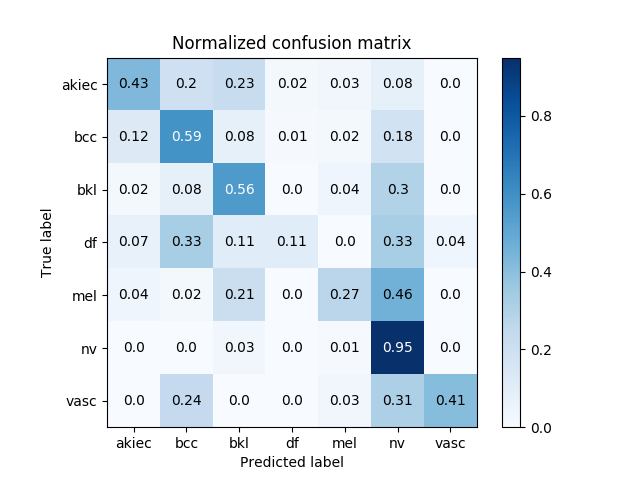
\includegraphics[width=15cm]{images/firstMatrix.png}
			\caption{Confusion matrix of the proposed model}
			\label{fig:first-matrix}
		\end{figure}
		
		It is possible to see that our model has difficulties in predicting Dermatofibromas (only 11\% correctly classified) and Melanomas (only 27\% correctly classified). In particular, Dermatofibromas are confused with Basal cell carcinomas (33\% of Dermatofibromas are classified like a Basal cell carcinoma) and Melanocytic nevis (33\% of Dermatofibromas are classified like a Melanocytic nevi), while Melanomas are confused with Melanocytic nevis (46\% of Melanomas are classified like a Melanocytic nevi). 
		This means that these classes are similar in terms of features and the imbalanced of the dataset does not help in discriminating well between them. We have too few examples for Dermatofibromas and too much examples for Melanocytic Nevis. Similar problems are also present in few of the other classes.
				
			
		
		
		
		
		
		
		